% Progressive Fee Curve Diagram
% Shows fee multiplier as a function of cluster wealth percentile
%
% ACCESSIBILITY ALT TEXT:
% A line graph showing progressive fee structure. X-axis shows wealth
% percentile (0-100%), Y-axis shows fee multiplier (1x-6x). The curve is
% flat at 1x for bottom 50%, rises gently to 1.5x at 70%, steeper to 3x at
% 90%, then sharply to 6x for top 1%. Shaded regions show increasing fee
% intensity. Vertical dashed lines mark 50%, 90%, and 99% thresholds. The
% design ensures typical users pay base fees while wealth concentration
% faces economic pressure through higher transaction costs.

\begin{figure}[ht]
\centering
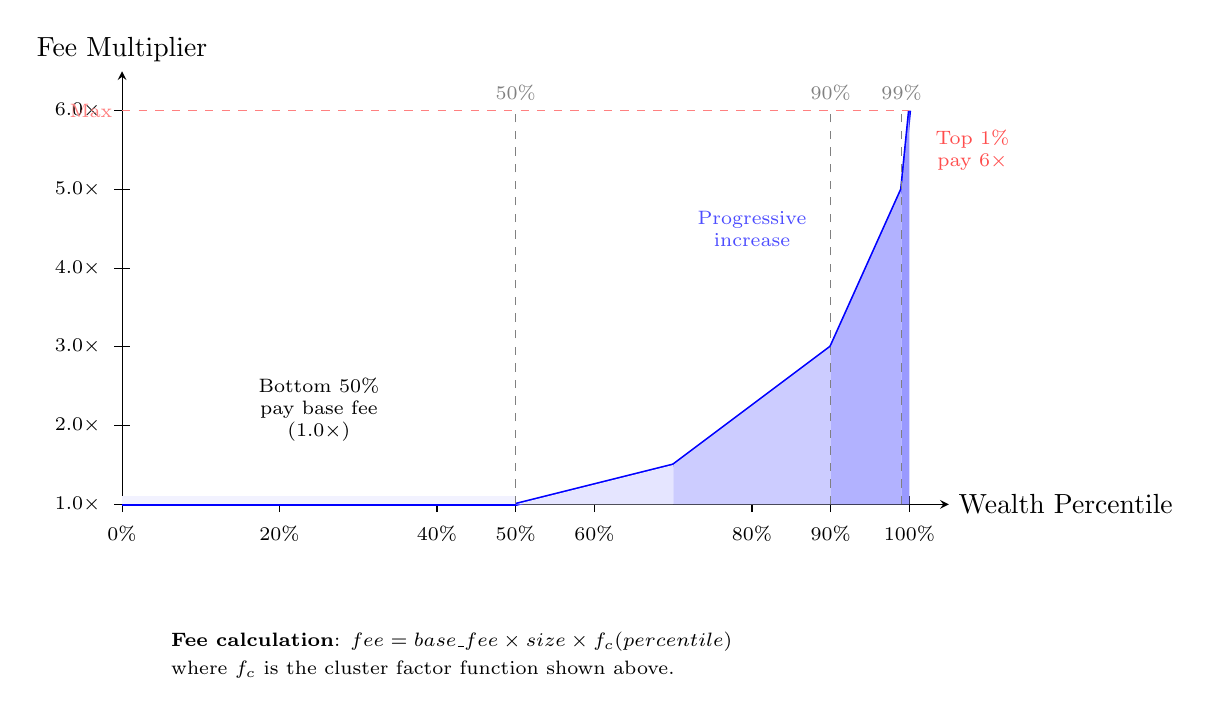
\begin{tikzpicture}[
    scale=1,
    >=stealth,
]

% Axes
\draw[->] (0,0) -- (10.5,0) node[right] {Wealth Percentile};
\draw[->] (0,0) -- (0,5.5) node[above] {Fee Multiplier};

% Y-axis labels
\foreach \y/\label in {0/1.0$\times$, 1/2.0$\times$, 2/3.0$\times$, 3/4.0$\times$, 4/5.0$\times$, 5/6.0$\times$} {
    \draw (-0.1,\y) -- (0.1,\y);
    \node[left] at (-0.15,\y) {\scriptsize \label};
}

% X-axis labels
\foreach \x/\label in {0/0\%, 2/20\%, 4/40\%, 5/50\%, 6/60\%, 8/80\%, 9/90\%, 10/100\%} {
    \draw (\x,-0.1) -- (\x,0.1);
    \node[below] at (\x,-0.15) {\scriptsize \label};
}

% Progressive fee curve (piecewise linear approximation of sigmoid-like curve)
% Bottom 50%: flat at 1x
\draw[very thick, blue] (0,0) -- (5,0);
% 50-70%: gentle rise to 1.5x
\draw[very thick, blue] (5,0) -- (7,0.5);
% 70-90%: steeper rise to 3x
\draw[very thick, blue] (7,0.5) -- (9,2);
% 90-99%: steep rise to 5x
\draw[very thick, blue] (9,2) -- (9.9,4);
% Top 1%: max at 6x
\draw[very thick, blue] (9.9,4) -- (10,5);

% Fill regions with gradient-like shading
\fill[blue!5] (0,0) rectangle (5,0.1);
\fill[blue!10] (5,0) -- (7,0.5) -- (7,0) -- cycle;
\fill[blue!20] (7,0) -- (7,0.5) -- (9,2) -- (9,0) -- cycle;
\fill[blue!30] (9,0) -- (9,2) -- (9.9,4) -- (9.9,0) -- cycle;
\fill[blue!40] (9.9,0) -- (9.9,4) -- (10,5) -- (10,0) -- cycle;

% Key percentile markers
\draw[dashed, gray] (5,0) -- (5,5);
\node[above, font=\scriptsize, gray] at (5,5) {50\%};

\draw[dashed, gray] (9,0) -- (9,5);
\node[above, font=\scriptsize, gray] at (9,5) {90\%};

\draw[dashed, gray] (9.9,0) -- (9.9,5);
\node[above, font=\scriptsize, gray] at (9.9,5) {99\%};

% Annotations
\node[align=center, font=\scriptsize] at (2.5,1.2) {Bottom 50\%\\pay base fee\\(1.0$\times$)};

\node[align=center, font=\scriptsize, blue!70] at (8,3.5) {Progressive\\increase};

\node[align=center, font=\scriptsize, red!70] at (10.8,4.5) {Top 1\%\\pay 6$\times$};

% Horizontal reference line at 6x
\draw[dashed, red!50] (0,5) -- (10,5);
\node[left, font=\scriptsize, red!50] at (0,5) {Max};

% Formula
\node[align=left, font=\scriptsize, anchor=north west] at (0.5,-1.5) {
    \textbf{Fee calculation}: $\text{fee} = \text{base\_fee} \times \text{size} \times f_c(\text{percentile})$\\[2pt]
    where $f_c$ is the cluster factor function shown above.
};

\end{tikzpicture}
\caption{Progressive fee multiplier based on cluster wealth percentile. Users in
the bottom 50\% of wealth distribution pay the base fee (1$\times$). Fees increase
progressively for wealthier clusters, reaching maximum 6$\times$ for the top 1\%.
This creates Sybil-resistant economic pressure against wealth concentration while
remaining minimal for typical users.}
\label{fig:progressive-fee}
\end{figure}
